\documentclass[tikz,border=2pt]{standalone}
\usepackage{amsmath}
\usepackage{fontspec}
\usepackage{unicode-math}
\setmainfont{Libertinus Serif}
\setsansfont{Libertinus Sans}
\setmathfont{Libertinus Math}[Scale=MatchUppercase]
\setmonofont{JetBrains Mono}[Scale=MatchLowercase,RawFeature={-liga,-calt,-clig,-dlig}]
\newfontface\figurekwface{JetBrains Mono SemiBold}[Scale=MatchLowercase,RawFeature={-liga,-calt,-clig,-dlig}]
\newcommand{\figurekw}[1]{{\figurekwface #1}}
\usetikzlibrary{positioning,arrows.meta,fit,backgrounds,calc}

\newcommand{\Z}{\mathbb{Z}}

\definecolor{ink}{HTML}{16191D}
\definecolor{accent}{HTML}{1F4E79}
\definecolor{accentsoft}{HTML}{E8EEF4}
\definecolor{accentwarm}{HTML}{9A5B00}
\definecolor{accentplum}{HTML}{8E2F5F}
\definecolor{muted}{HTML}{5B6470}
\definecolor{hairline}{HTML}{C9CFD6}

\tikzset{
  house/.style={
    >={Stealth[length=2.1mm, width=1.6mm]},
    line width=0.5pt,
    node distance=9mm and 15mm,
    every node/.style={font=\small},
  },
  box/.style={
    draw=ink, line width=0.5pt, rounded corners=1.5pt,
    inner xsep=6pt, inner ysep=4pt, align=center,
  },
  boxhi/.style={box, draw=accent, fill=accentsoft, text=ink},
  boxdim/.style={box, draw=hairline, text=muted},
  flow/.style={->, draw=ink},
  flowdim/.style={->, draw=hairline},
  lbl/.style={font=\footnotesize\itshape, text=accent, inner sep=2pt},
  lbldim/.style={font=\footnotesize, text=muted, inner sep=2pt},
  group/.style={draw=hairline, dashed, rounded corners=2pt, inner sep=7pt},
}

\definecolor{loanink}{HTML}{8C4A2F}
\definecolor{returnink}{HTML}{007A59}
\definecolor{returnsoft}{HTML}{DAF1E9}
\begin{document}
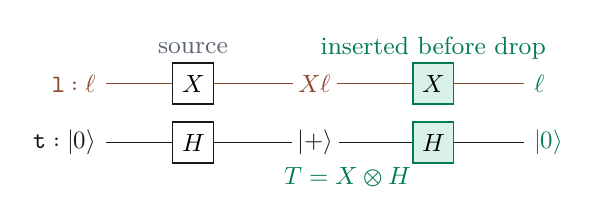
\begin{tikzpicture}[house,semithick,font=\normalsize,
 gate/.style={draw=ink,fill=white,minimum width=5.2mm,minimum height=5.2mm,inner sep=1.5pt},
 repair/.style={gate,draw=returnink,fill=returnsoft}]
\node[font=\small,text=muted] at (1.15,.7) {source};
\node[font=\small,text=returnink] at (4.2,.7) {inserted before drop};
\foreach \y/\initial/\middle/\last/\op/\wirecolour in {.25/{\text{\texttt{l}}:\ell}/{X\ell}/{\ell}/X/loanink,-.50/{\text{\texttt{t}}:|0\rangle}/{|+\rangle}/{|0\rangle}/H/ink}{
 \node[anchor=east,text=\wirecolour,inner sep=2pt] at (0,\y) {$\initial$};
 \draw[\wirecolour] (0.05,\y)--(5.35,\y);
 \node[gate] at (1.15,\y) {$\op$};
 \node[fill=white,text=\wirecolour,inner sep=2pt] at (2.7,\y) {$\middle$};
 \node[repair] at (4.2,\y) {$\op$};
 \node[anchor=west,text=returnink,inner sep=2pt] at (5.4,\y) {$\last$};
}
\node[text=returnink,font=\small] at (3.1,-.94) {$T=X\otimes H$};
\end{tikzpicture}
\end{document}
